% global-visibility-commit.tex

\documentclass{standalone}
% newcommands.tex

\newcommand{\enq}{\texttt{enq}}
\newcommand{\deq}{\texttt{deq}}
\newcommand{\pput}{\texttt{PUT}}
\newcommand{\get}{\texttt{GET}}
\newcommand{\vs}{\texttt{vis}}
\newcommand{\so}{\texttt{so}}
\newcommand{\arb}{\texttt{ar}}
\newcommand{\rf}{\texttt{rf}}

% example
\newcommand{\po}[2]{\draw [->, thick] (#1) to node[above] {\Large{\so}} (#2);}
\newcommand{\pva}[2]{\draw [->, thick] (#1) to node[above] {$\Large{\so},\Large{\vs},\Large{\arb}$} (#2);}
\newcommand{\pbva}[2]{\draw [->, thick] (#1) to node[above] {$\Large{\so}$} node[below] {$\Large{\vs},\Large{\arb}$} (#2);}
\newcommand{\pv}[2]{\draw [->, thick] (#1) to node[above] {\Large{\so}} node[below] {\Large{\vs}} (#2);}
\newcommand{\evis}[2]{\draw [->, thick] (#1) to node[above, sloped, near end] {\Large{\vs}} (#2);}
\newcommand{\mvis}[2]{\draw [->, thick] (#1) to node[above, sloped] {\Large{\vs}} (#2);}
\newcommand{\ar}[2]{\draw [->, thick, allow upside down] (#1) to node[above, sloped] {\Large{\arb}} (#2);}
\newcommand{\va}[2]{\draw [->, thick, allow upside down] (#1) to node[above, sloped] {$\Large{\vs},\Large{\arb}$} (#2);}
\newcommand{\vab}[2]{\draw [->, thick, allow upside down] (#1) to node[below, sloped, near end] {$\Large{\vs},\Large{\arb}$} (#2);}
\newcommand{\vae}[2]{\draw [->, thick, allow upside down] (#1) to node[above, sloped, near end] {$\Large{\vs},\Large{\arb}$} (#2);}
\newcommand{\vas}[2]{\draw [->, thick, allow upside down] (#1) to node[sloped, near start, above] {$\Large{\vs},\Large{\arb}$} (#2);}

% serialization
\newcommand{\scc}[2]{\draw [->, very thick] (#1) to (#2);}
\newcommand{\rva}[2]{\draw [->, thick, allow upside down] (#1) to node[above, sloped] {$\Large{\rf},\Large{\vs},\Large{\arb}$} (#2);}
\newcommand{\rvb}[2]{\draw [->, thick, allow upside down] (#1) to node[below, sloped] {$\Large{\rf},\Large{\vs},\Large{\arb}$} (#2);}


\usepackage{tikz}
\usetikzlibrary{calc, shapes, positioning,
  arrows.meta, decorations.pathmorphing}

\begin{document}
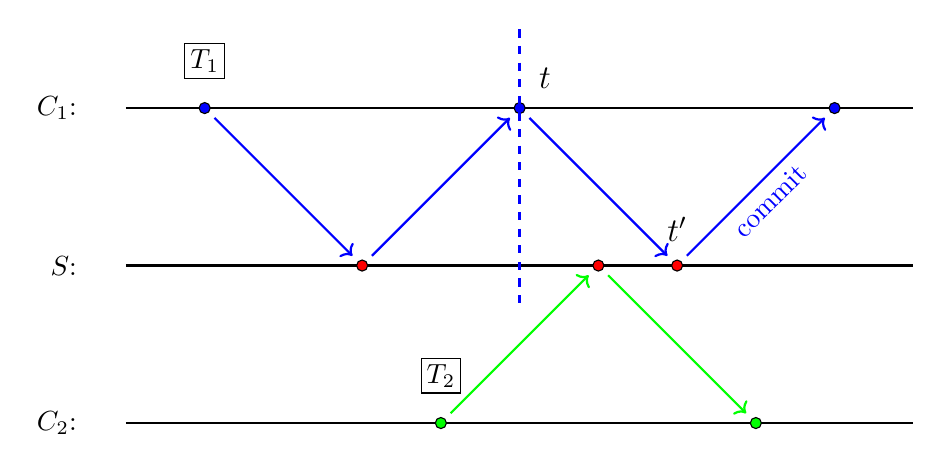
\begin{tikzpicture}[
  msg/.style = {->, thick},
  client/.style = {thick},
  txn/.style = {draw, inner sep = 2pt}]

  % c1
  \coordinate (c1-start) at (0,0);
  \coordinate (c1-end) at (10,0);
  \draw[client] (c1-start) to (c1-end);
  \node[left = 0.50cm of c1-start] (c1) {$C_{1}$:};

  \node (c1-10) at ($(c1-start)!0.10!(c1-end)$) {};
  \node (c1-50) at ($(c1-start)!0.50!(c1-end)$) {};
  \node (c1-90) at ($(c1-start)!0.90!(c1-end)$) {};

  \node[txn, above = 0.25cm of c1-10] (t1) {$T_{1}$};

  \draw[fill=blue] (c1-10) circle [radius=2pt] node[above] {};
  \draw[fill=blue] (c1-50) circle [radius=2pt] node[above right = 5pt, font = \large] {$t$};
  \draw[fill=blue] (c1-90) circle [radius=2pt] node[above] {};

  % s
  \coordinate (s-start) at (0, -2);
  \coordinate (s-end) at (10, -2);
  \draw[client] (s-start) to (s-end);
  \node[left = 0.50cm of s-start] (s) {$S$:};

  \node (s-30) at ($(s-start)!0.30!(s-end)$) {};
  \node (s-60) at ($(s-start)!0.60!(s-end)$) {};
  \node (s-70) at ($(s-start)!0.70!(s-end)$) {};

  \draw[fill=red] (s-30) circle [radius=2pt] node[above] {};
  \draw[fill=red] (s-60) circle [radius=2pt] node[above] {};
  \draw[fill=red] (s-70) circle [radius=2pt] node[above = 5pt, font = \large] {$t'$};

  % c2
  \coordinate (c2-start) at (0, -4);
  \coordinate (c2-end) at (10, -4);
  \draw[client] (c2-start) to (c2-end);
  \node[left = 0.50cm of c2-start] (c2) {$C_{2}$:};

  \node (c2-40) at ($(c2-start)!0.40!(c2-end)$) {};
  \node (c2-80) at ($(c2-start)!0.80!(c2-end)$) {};

  \node[txn, above = 0.25cm of c2-40] (t2) {$T_{2}$};

  \draw[fill=green] (c2-40) circle [radius=2pt] node[above] {};
  \draw[fill=green] (c2-80) circle [radius=2pt] node[above] {};

  \coordinate (above) at ($(c1-50) + (0, 1.0cm)$);
  \coordinate (below) at ($(c1-50) + (0, -2.5cm)$);
  \draw[dashed, blue, very thick] (above) to (below);

  % c1 <-> s
  \draw[msg, blue] (c1-10) to (s-30);
  \draw[msg, blue] (s-30) to (c1-50);
  \draw[msg, blue] (c1-50) to (s-70);
  \draw[msg, blue] (s-70) to node[sloped, below] {commit} (c1-90);

  % c2 <-> s
  \draw[msg, green] (c2-40) to (s-60);
  \draw[msg, green] (s-60) to (c2-80);
\end{tikzpicture}
\end{document}